\documentclass[11pt,a4paper]{article}
\usepackage[margin=2.5cm]{geometry}
\usepackage{graphicx}
\usepackage{booktabs}
\usepackage{hyperref}
\usepackage{amsmath}
\usepackage{caption}
\usepackage{subcaption}
\usepackage{float}
\usepackage{xcolor}
\usepackage{listings}
\usepackage{cite}
\usepackage{array}
\usepackage{multirow}

\hypersetup{colorlinks=true, linkcolor=blue, citecolor=blue, urlcolor=blue}

\title{\textbf{HC701 -- Assignment 2}\\
       CT Lung Analysis and Chest X-ray Pneumonia Classification}
\author{Mashrafi Monon}
\date{\today}

\begin{document}
\maketitle
\tableofcontents
\newpage

% ─────────────────────────────────────────────────────────────────────────────
\section{Task 1: CT Lung Analysis}
% ─────────────────────────────────────────────────────────────────────────────

\subsection{Task 1.1 -- DICOM Inspection and NIfTI Extraction}

The dataset consists of a series of chest CT DICOM slices. Each filename encodes
the slice identity via the DICOM \texttt{InstanceNumber} tag. Slices 71--110 were
extracted using \texttt{pydicom}, stacked along the z-axis to form a 3-D volume
of shape $512 \times 512 \times 40$, and saved as a compressed NIfTI file
(\texttt{.nii.gz}) using \texttt{nibabel}.

\begin{table}[H]
\centering
\caption{Extracted volume properties}
\begin{tabular}{ll}
\toprule
\textbf{Property} & \textbf{Value} \\
\midrule
Slices extracted    & 71--110 (40 slices) \\
Volume shape        & $512 \times 512 \times 40$ \\
Pixel spacing       & $0.684 \times 0.684$ mm \\
Slice thickness     & 1.25 mm \\
Voxel volume        & $5.84 \times 10^{-4}$ cm$^3$ \\
Output format       & NIfTI (.nii.gz) \\
\bottomrule
\end{tabular}
\end{table}

The affine matrix was constructed from the pixel spacing and slice thickness
metadata, ensuring correct physical dimensions in downstream tools.
Figure~\ref{fig:slicer_volume} shows the volume loaded in 3D Slicer.

\begin{figure}[H]
    \centering
    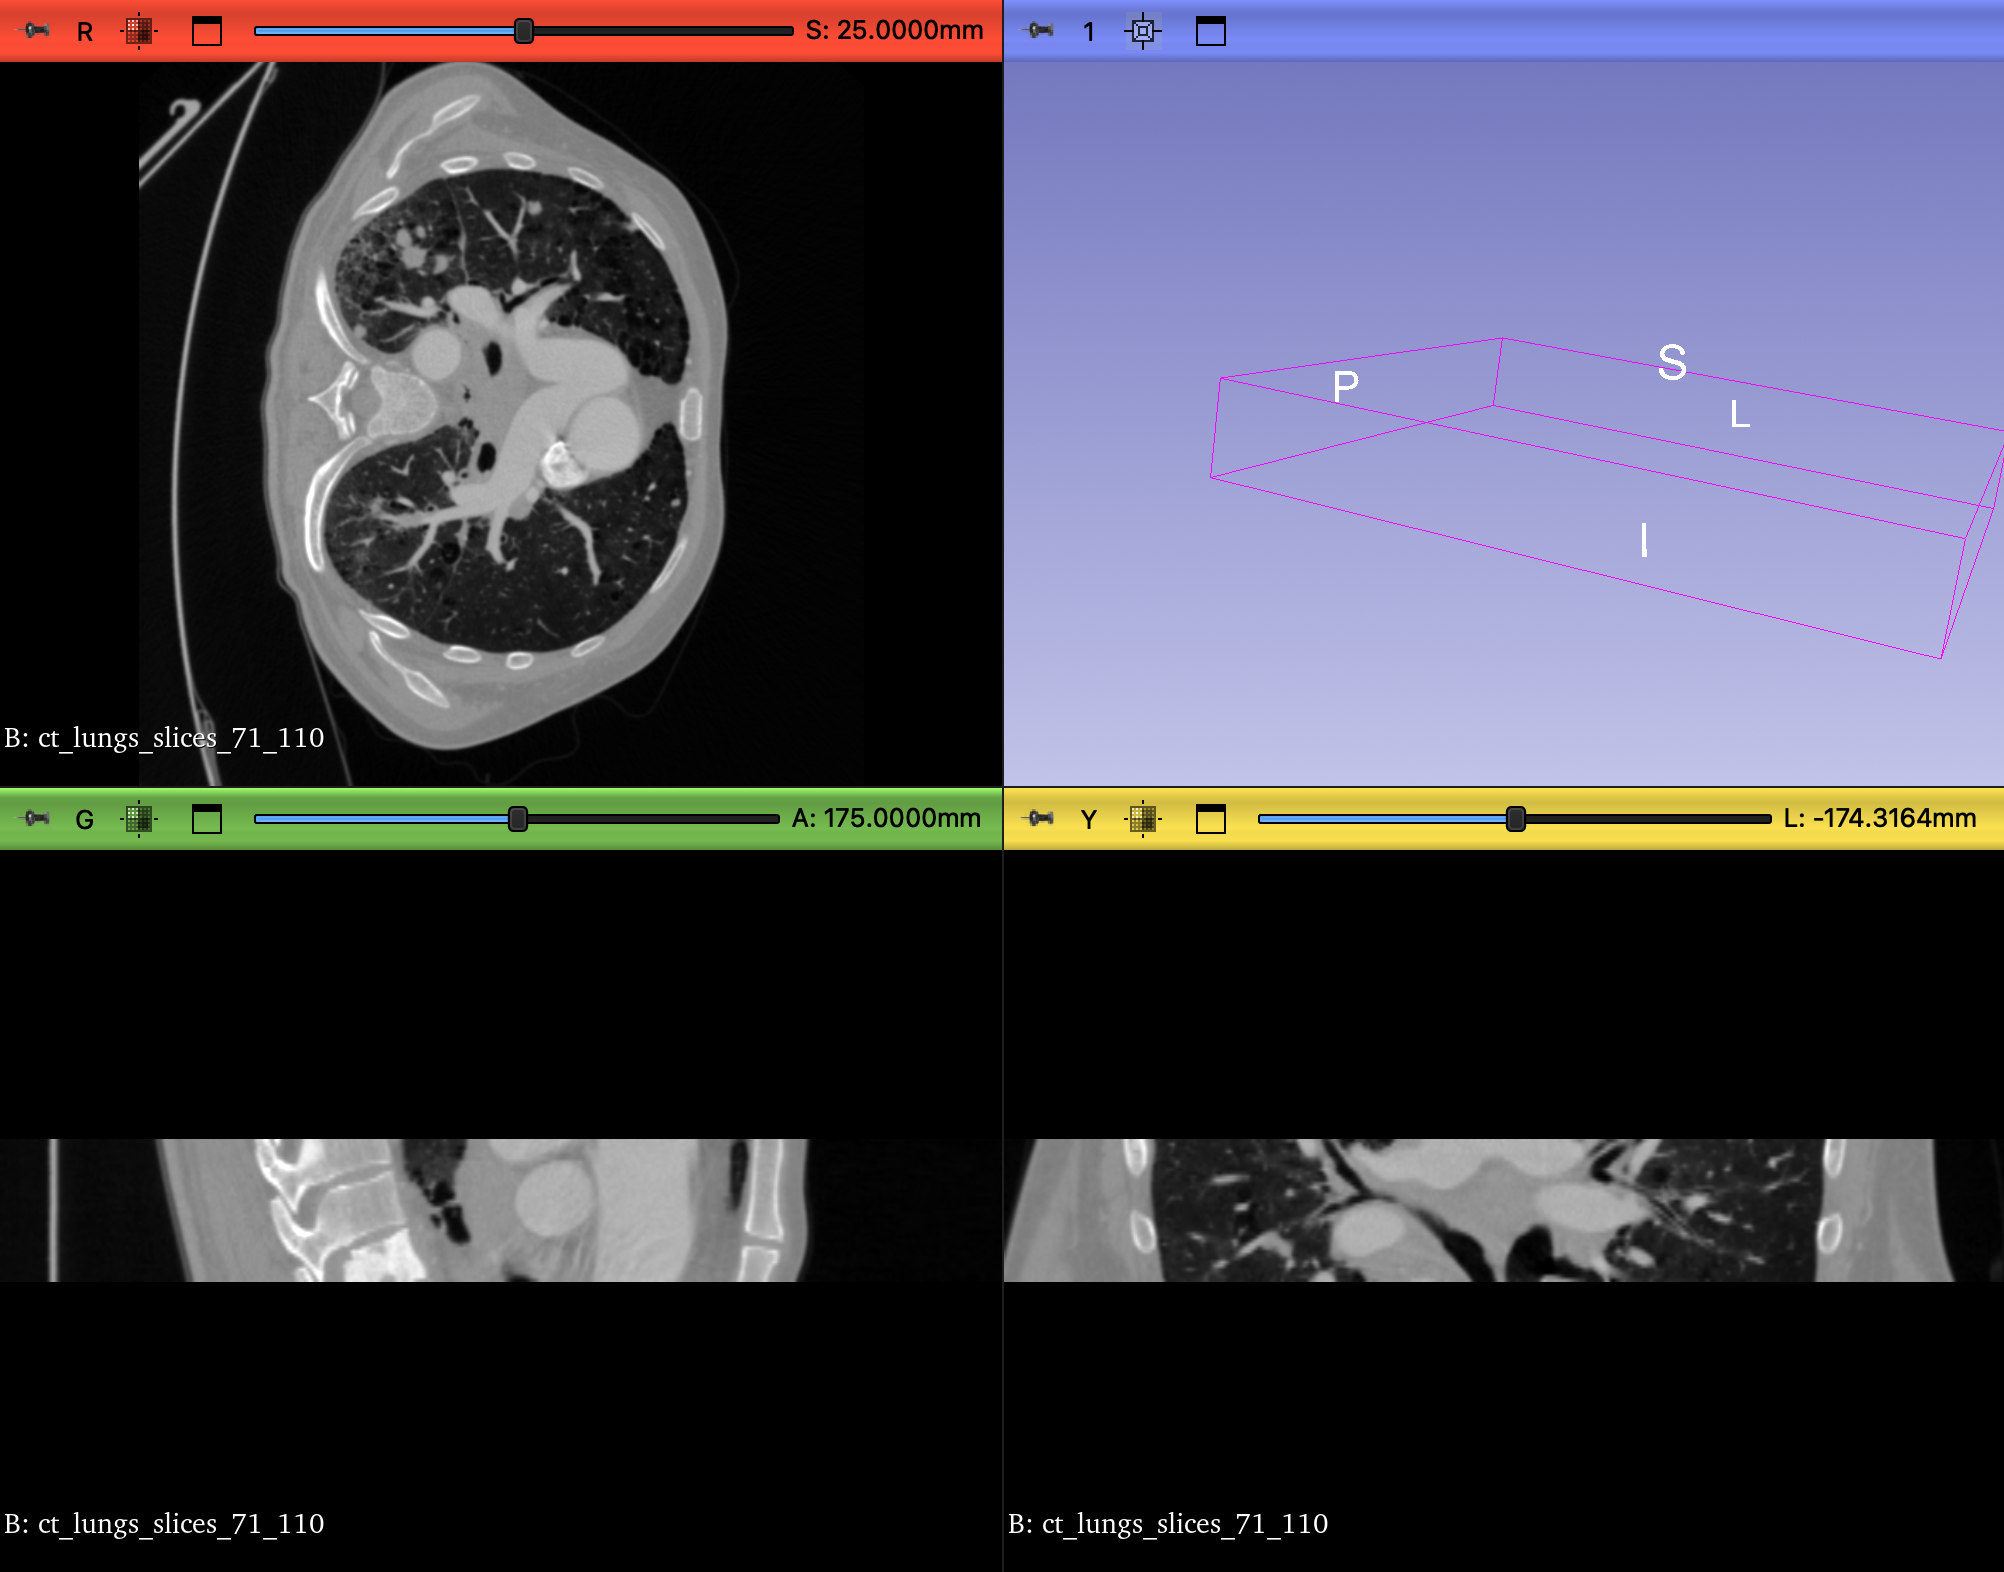
\includegraphics[width=0.8\linewidth]{task1_1_volume_slicer.png}
    \caption{CT volume (slices 71--110) loaded in 3D Slicer, showing axial,
             coronal, and sagittal views.}
    \label{fig:slicer_volume}
\end{figure}

% ─────────────────────────────────────────────────────────────────────────────
\subsection{Task 1.2 -- Optimal Intensity Window}

CT images are displayed using a \emph{window/level} scheme that maps a selected
HU range to the 0--255 display range. Tissue outside the range is clipped to
black or white. Because the NIfTI volume stores raw DICOM pixel values (not
Hounsfield Units), the standard lung window (centre $-600$ HU, width 1500 HU)
was converted to the raw value scale by adding the scanner's rescale intercept.
The effective raw-value window used was:

\begin{itemize}
    \item \textbf{Window Width:} 1200
    \item \textbf{Window Centre (Level):} 600
    \item \textbf{Display range:} 0 -- 1200 raw pixel units
\end{itemize}

This range maps background air to black, lung parenchyma to dark grey, soft
tissue to mid-grey, and bone to white -- identical to the clinical standard
lung window \cite{kanne2012chest}. Six preset windows (brain, mediastinum, lung,
bone, liver, wide) were evaluated; the lung window produced the clearest
delineation of parenchymal structure.

\begin{figure}[H]
    \centering
    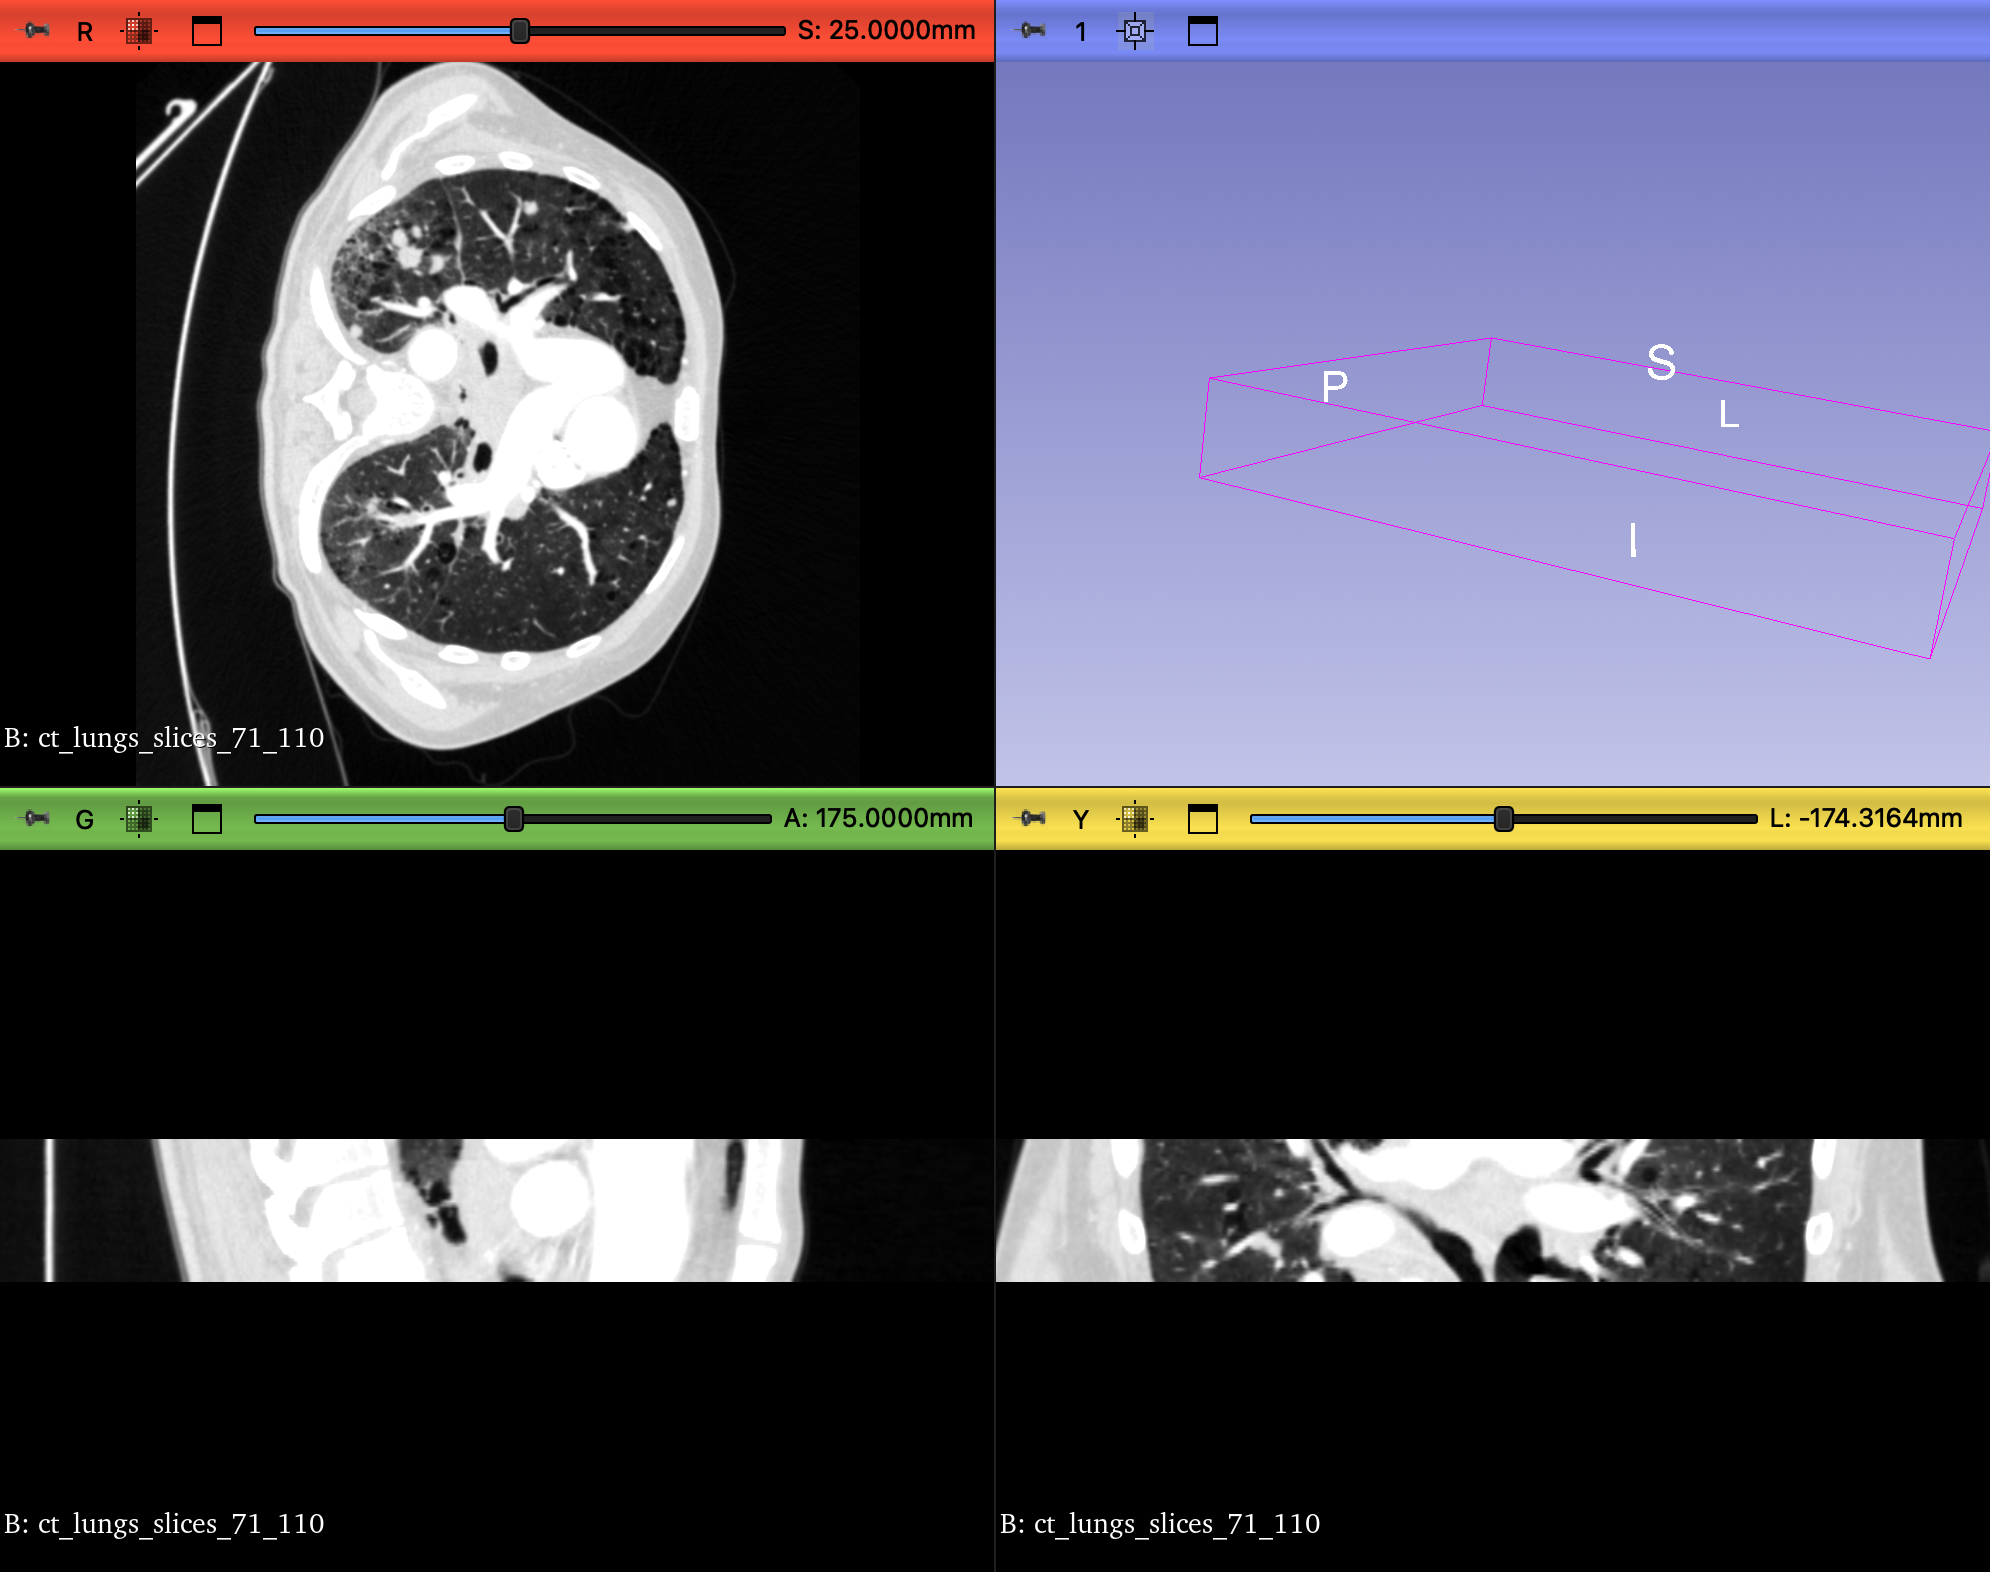
\includegraphics[width=0.9\linewidth]{task1_2_volume_slicer.png}
    \caption{Optimal lung window (W:1200, L:600) applied in 3D Slicer. Left
             to right: axial, coronal, and sagittal views. Lung air-spaces
             appear dark grey against brighter chest-wall tissue.}
    \label{fig:slicer_window}
\end{figure}

% ─────────────────────────────────────────────────────────────────────────────
\subsection{Task 1.3 -- Lung Segmentation (Non-ML)}

\subsubsection{Method}

A classical, non-machine-learning pipeline was implemented in Python using
\texttt{scipy.ndimage} and \texttt{scikit-image}. The steps are as follows:

\paragraph{Step 1 -- Intensity thresholding.}
All voxels with raw pixel value below a threshold of 400 are classified as
``air-like.'' This captures both the external background air surrounding the
patient and the internal lung air-spaces. The threshold was chosen empirically
from the raw value histogram: lung air occupies values 0--300, soft tissue
300--1100, and bone above 1100.

\paragraph{Step 2 -- Per-slice 2D flood-fill to remove external background.}
A 3-D flood-fill from the volume border fails for thoracic CT because the trachea
and main bronchi form a continuous air path between the lung interior and the
superior image border. Instead, a \emph{2-D} connected-component flood-fill is
applied independently to each axial slice. Within each slice, any air-like
connected component that touches the image edge is classified as external
background and discarded. The remaining internal components correspond to
the intra-pulmonary air spaces.

\paragraph{Step 3 -- Morphological refinement.}
Binary closing with a disk structuring element (radius 3 pixels) fills small
intra-parenchymal holes. Small spurious objects smaller than 500 voxels are
removed. A single dilation/erosion pass (iterations~$= 1$) smooths boundaries
without appreciably shrinking the lung regions \cite{gonzalez2018digital}.

\paragraph{Step 4 -- Connected-component labelling and left/right separation.}
The two largest connected components per slice are retained. Left and right lungs
are distinguished by the x-centroid of each component: the component whose
centroid lies to the left of the image midline is labelled \emph{left lung}
(label~1), and the other is labelled \emph{right lung} (label~2).

\paragraph{Step 5 -- Volume computation.}
Voxel volume is $v = 0.684 \times 0.684 \times 1.25 = 5.84 \times 10^{-4}$
cm$^3$. Lung volume in cm$^3$ is the voxel count multiplied by $v$.

\subsubsection{Results}

\begin{table}[H]
\centering
\caption{Lung volume measurements (slices 71--110)}
\begin{tabular}{lrr}
\toprule
\textbf{Region} & \textbf{Voxel count} & \textbf{Volume (cm$^3$)} \\
\midrule
Left lung  & 976{,}382 & 570.33 \\
Right lung & 685{,}228 & 400.26 \\
Total      & 1{,}661{,}610 & 970.59 \\
\bottomrule
\end{tabular}
\end{table}

The slight asymmetry (left $>$ right) is plausible for this slice range: the
cardiac notch on the left is largely below the scan window, so the left lung
appears uncompressed, while the right lung shares the right hemithorax with the
liver dome visible in the lower slices.

\begin{figure}[H]
    \centering
    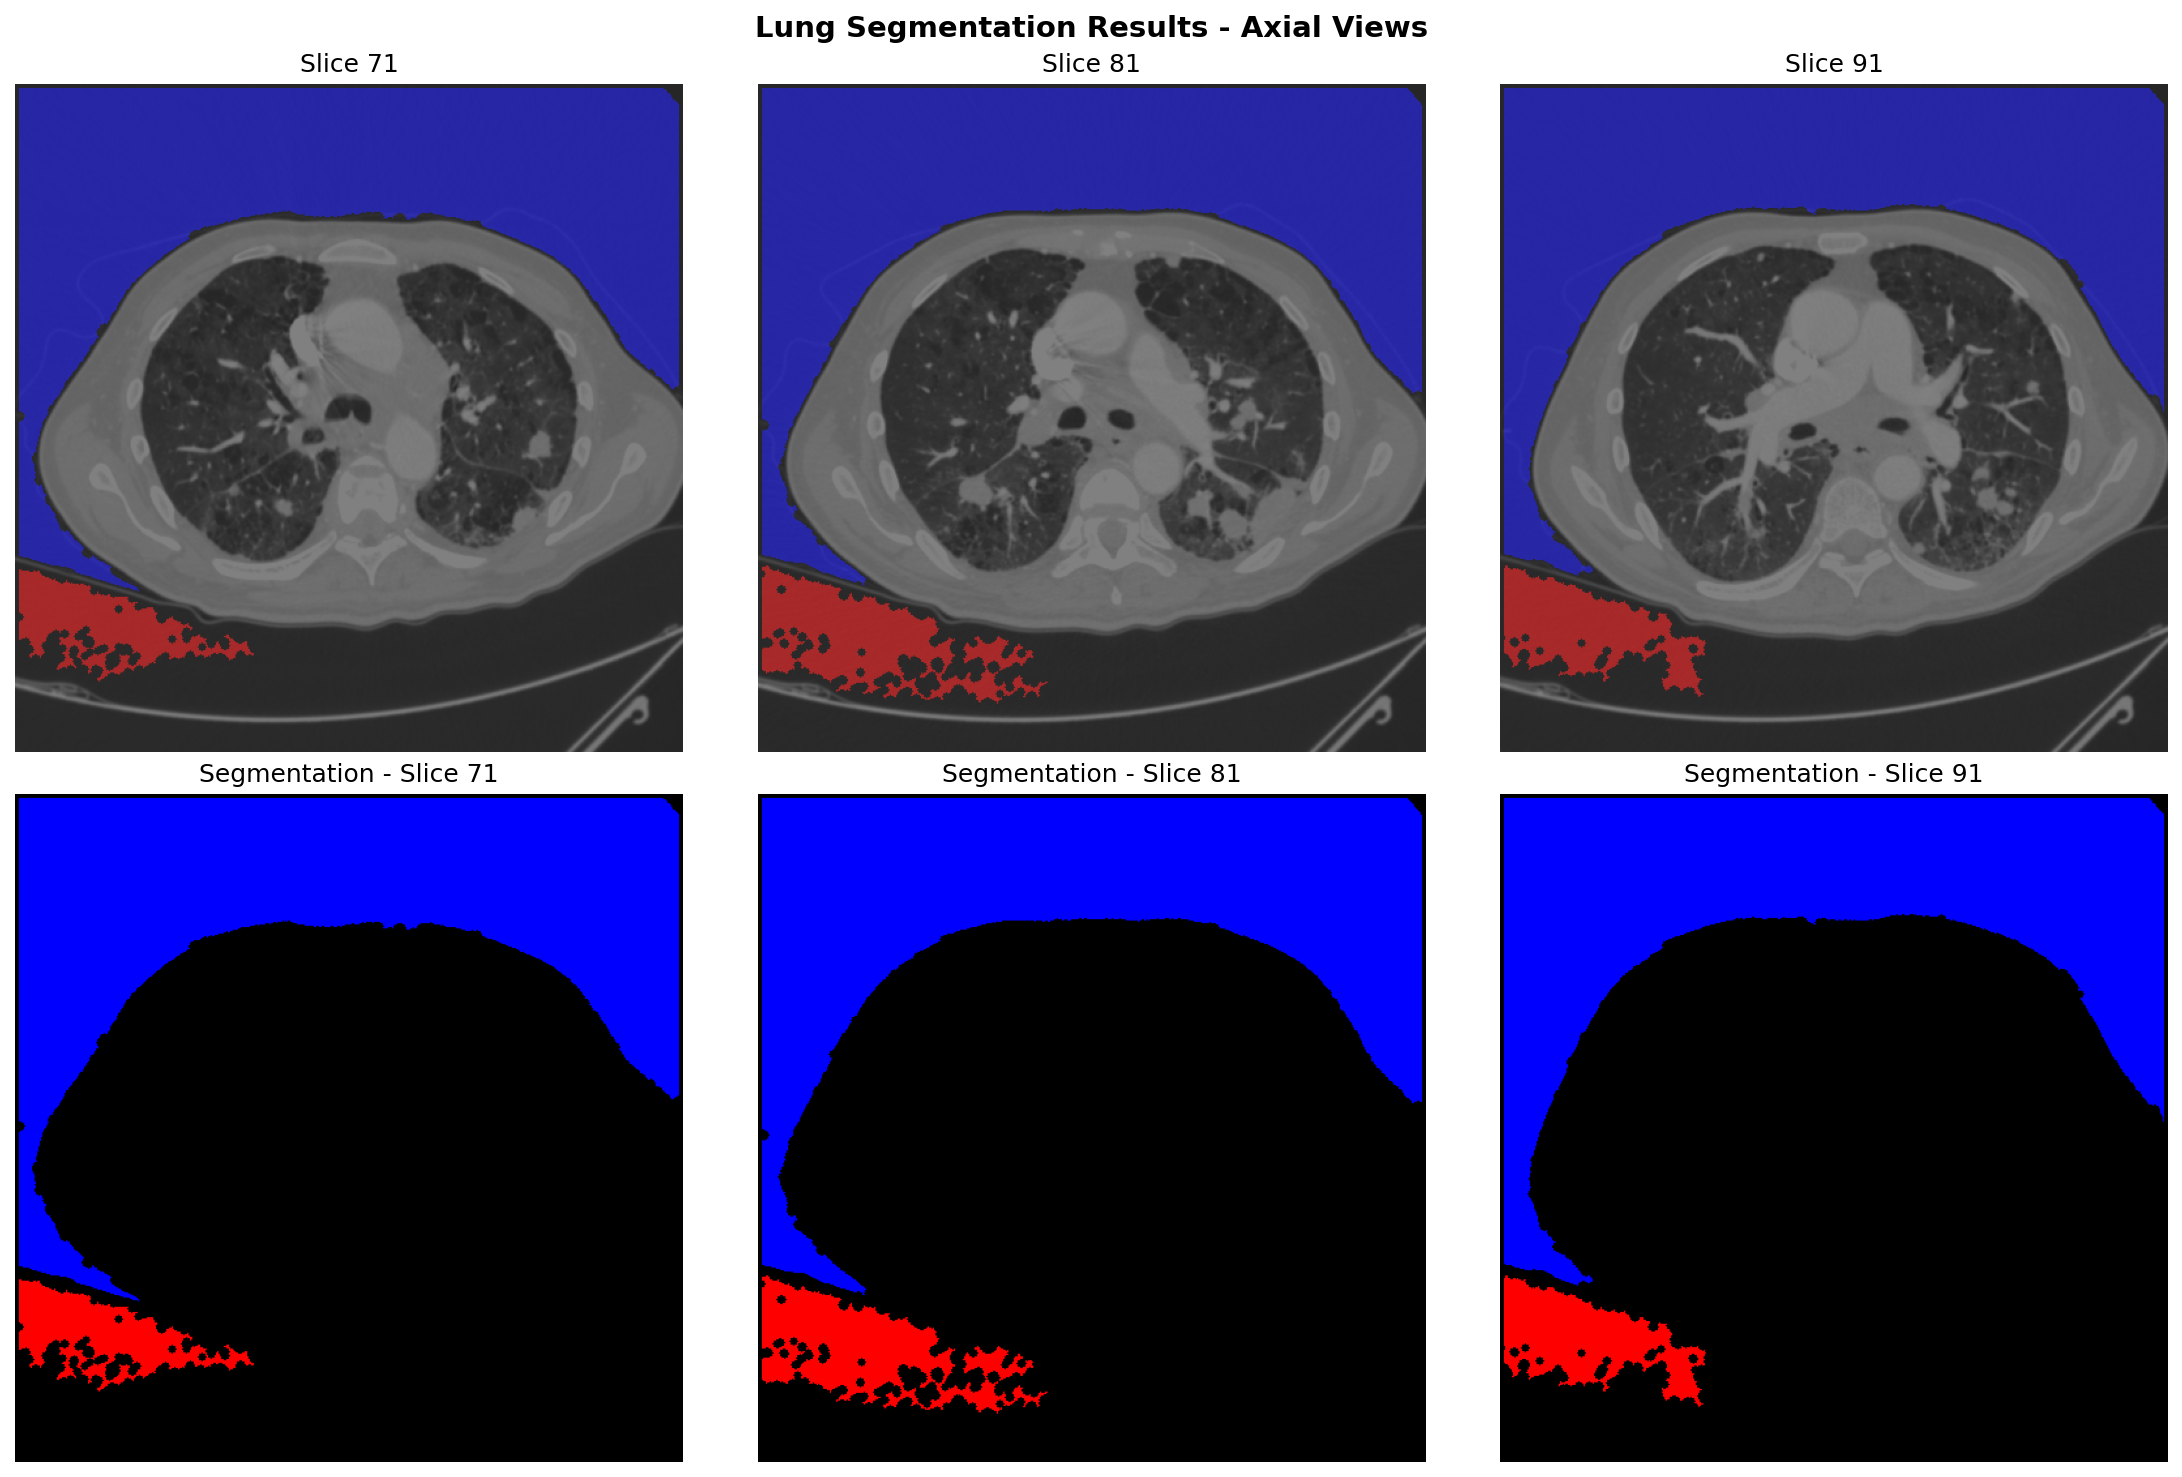
\includegraphics[width=0.9\linewidth]{segmentation_results/segmentation_axial_views.png}
    \caption{Segmentation results overlaid on axial slices. Red = left lung,
             blue = right lung.}
    \label{fig:seg_axial}
\end{figure}

\begin{figure}[H]
    \centering
    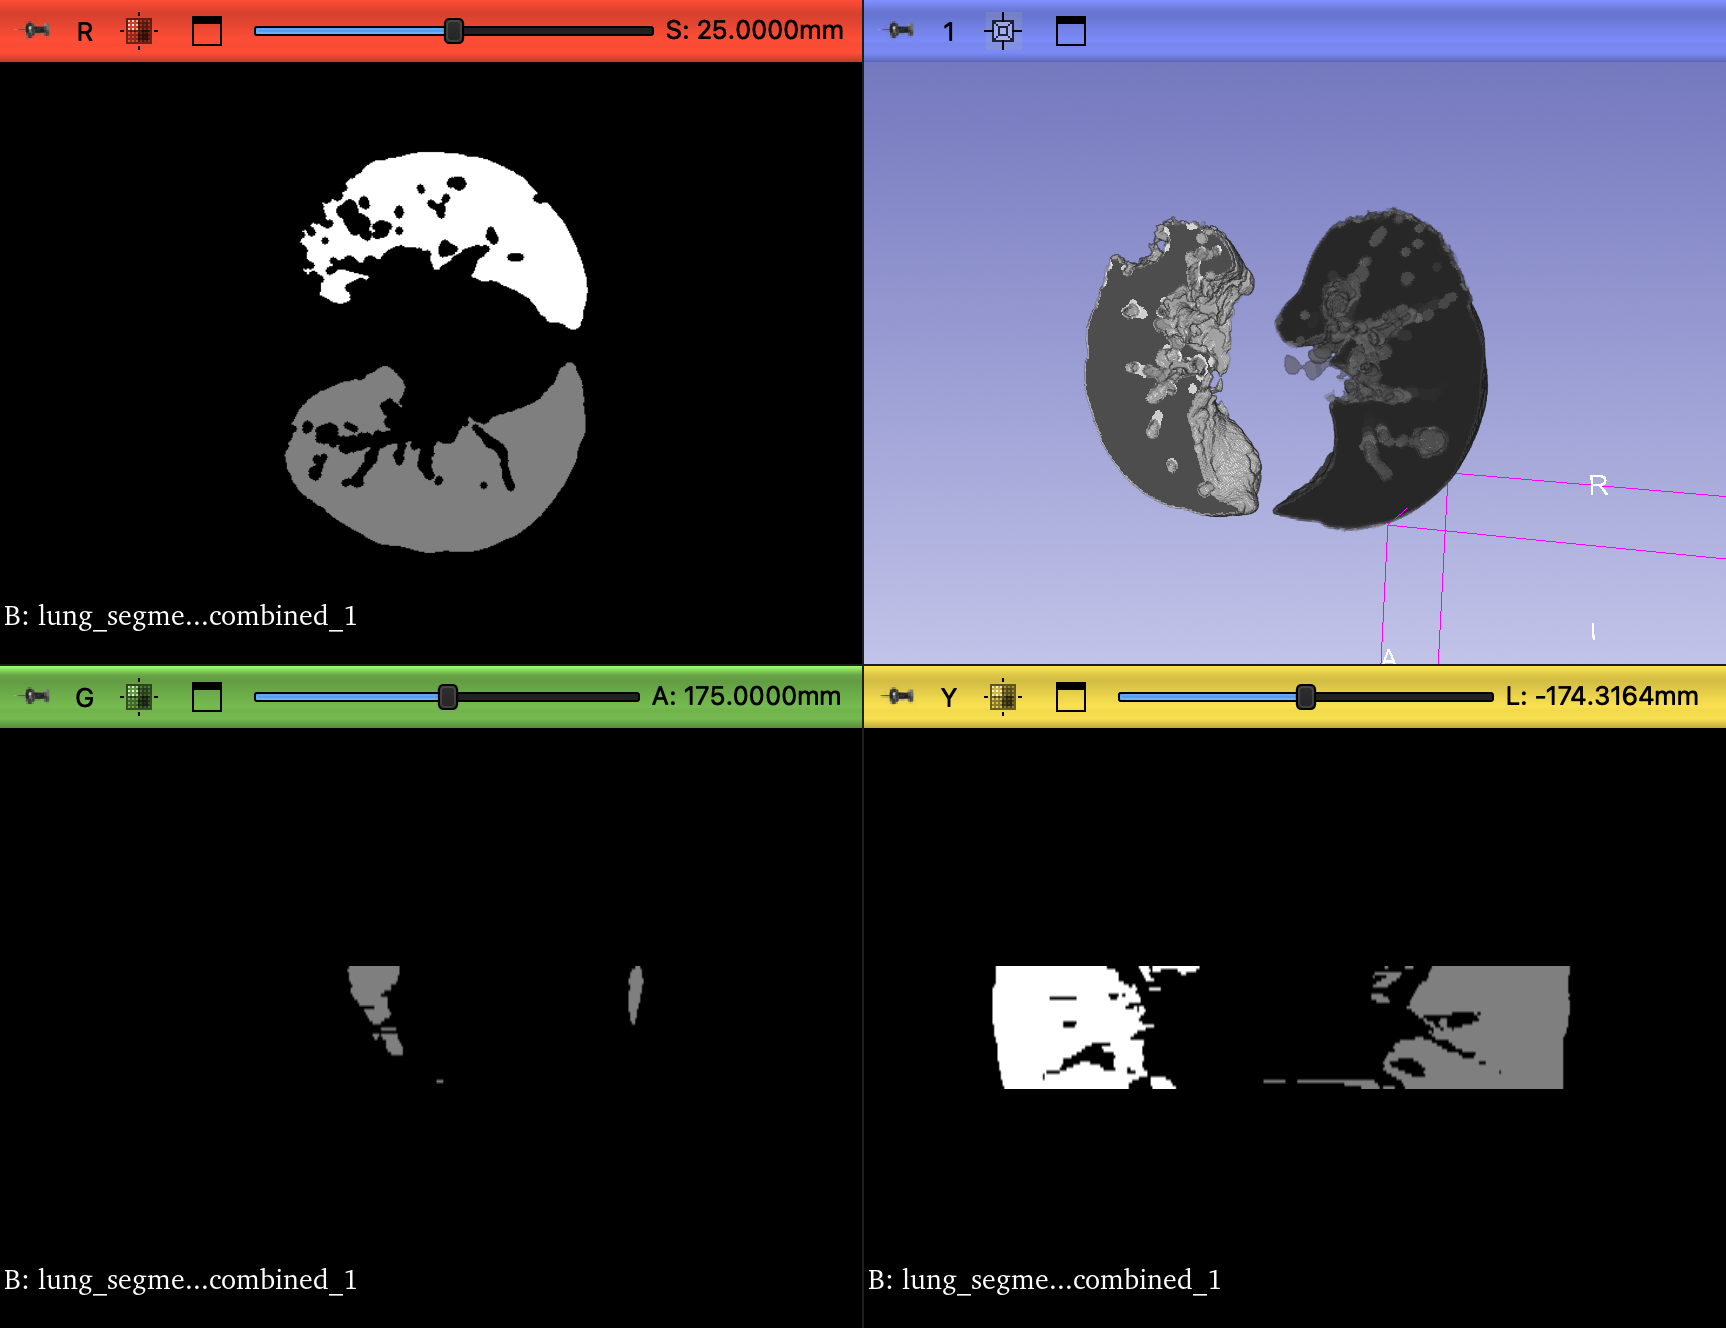
\includegraphics[width=0.8\linewidth]{task1_3_volume_slicer.png}
    \caption{3D surface rendering of the segmented lungs in 3D Slicer.}
    \label{fig:slicer_3d}
\end{figure}

% ─────────────────────────────────────────────────────────────────────────────
\newpage
\section{Task 2: Chest X-ray Pneumonia Classification}
% ─────────────────────────────────────────────────────────────────────────────

\subsection{Task 2.1 -- Dataset Preparation}

The Kaggle Chest X-ray Pneumonia dataset \cite{kermany2018labeled} contains
5{,}216 JPEG chest X-ray images organised into NORMAL and PNEUMONIA classes.
Only the original Kaggle \texttt{train/} split was used; it was re-partitioned
into training, validation, and test subsets using stratified sampling to
preserve the class ratio in every split (Table~\ref{tab:splits}).

\begin{table}[H]
\centering
\caption{Dataset splits (all drawn from the Kaggle training folder)}
\label{tab:splits}
\begin{tabular}{lrrr}
\toprule
\textbf{Split} & \textbf{NORMAL} & \textbf{PNEUMONIA} & \textbf{Total} \\
\midrule
Train (80\%) & 858  & 3{,}314 & 4{,}172 \\
Val   (10\%) & 108  & 414     & 522 \\
Test  (10\%) & 107  & 415     & 522 \\
\midrule
\textbf{Total} & \textbf{1{,}073} & \textbf{3{,}143} & \textbf{5{,}216} \\
\bottomrule
\end{tabular}
\end{table}

\paragraph{Class imbalance.}
The dataset is heavily imbalanced: 74.3\% PNEUMONIA vs.\ 25.7\% NORMAL.
This was addressed by setting
$\texttt{pos\_weight} = n_\text{NORMAL} / n_\text{PNEUMONIA} \approx 0.346$
in \texttt{BCEWithLogitsLoss}, which down-weights the majority class so that
misclassifying one NORMAL sample contributes equal gradient mass to
misclassifying one PNEUMONIA sample \cite{king2001logistic}.

\subsection{Task 2.2 -- ML Experiments}

\subsubsection{Data Augmentation}

Training images are augmented on-the-fly with:
\begin{itemize}
    \item \textbf{Random rotation} $\pm10^\circ$ -- accounts for patient
          positioning variation.
    \item \textbf{Random affine translation} up to 10\% in x and y -- simulates
          slight shifts in scan framing.
    \item \textbf{Colour jitter} (brightness $\pm0.2$, contrast $\pm0.2$) --
          mimics inter-scanner intensity variation.
    \item \textbf{Resize} to $224 \times 224$ pixels.
    \item \textbf{ImageNet normalisation} (mean $[0.485, 0.456, 0.406]$, std
          $[0.229, 0.224, 0.225]$) -- required for pretrained backbone
          compatibility \cite{krizhevsky2012imagenet}.
\end{itemize}
Validation and test images are only resized and normalised (no augmentation).

\subsubsection{Training Setup}

\begin{itemize}
    \item \textbf{Optimiser:} Adam \cite{kingma2014adam}, chosen because it
          adapts per-parameter learning rates and has been shown to converge
          reliably on medical image classification tasks \cite{rajpurkar2017chexnet}.
    \item \textbf{Loss:} \texttt{BCEWithLogitsLoss} with \texttt{pos\_weight}
          as described above.
    \item \textbf{LR scheduler:} ReduceLROnPlateau (factor 0.5, patience 3)
          halves the learning rate when validation loss stagnates.
    \item \textbf{Early stopping:} patience of 5 epochs on validation loss;
          the best checkpoint (lowest val loss) is restored via
          \texttt{copy.deepcopy} of the model state dict.
    \item \textbf{Gradient clipping:} max norm 1.0 to prevent occasional
          large gradient steps during fine-tuning.
    \item \textbf{Batch size:} 32. \textbf{Max epochs:} 50.
\end{itemize}

\subsubsection{Experiment Descriptions}

\begin{table}[H]
\centering
\caption{Summary of the five experiments}
\label{tab:experiments}
\renewcommand{\arraystretch}{1.4}
\begin{tabular}{>{\bfseries}p{0.5cm} p{3cm} p{2cm} p{7.5cm}}
\toprule
\textbf{Exp} & \textbf{Backbone} & \textbf{LR} & \textbf{Rationale} \\
\midrule
1 & Baseline CNN (4-layer custom) & 0.001 &
    A lightweight CNN trained from scratch establishes a lower-bound baseline.
    Designed with BatchNorm and Dropout (0.25/0.5) for regularisation
    \cite{lecun1998gradient}. \\

2 & ResNet50 \cite{he2016deep} (pretrained ImageNet) & 0.0001 &
    Deep residual connections allow gradients to flow through 50 layers without
    vanishing. A low LR (0.0001) is standard for fine-tuning to avoid
    destroying pretrained features \cite{yosinski2014transferable}.
    The final FC layer is replaced with a single sigmoid output. \\

3 & DenseNet121 \cite{huang2017densely} (pretrained ImageNet) & 0.0001 &
    DenseNet121 is the backbone of CheXNet \cite{rajpurkar2017chexnet}, which
    achieved radiologist-level pneumonia detection. Dense skip connections
    encourage feature reuse and are particularly effective on small medical
    datasets. \\

4 & EfficientNet-B3 \cite{tan2019efficientnet} (pretrained ImageNet) & 0.0001 &
    EfficientNet uses compound scaling (depth, width, resolution jointly) to
    achieve high accuracy at lower parameter counts than ResNet/DenseNet.
    B3 offers a strong accuracy/efficiency trade-off. \\

5 & DenseNet121 \cite{huang2017densely} (frozen backbone) & 0.001 &
    Ablation of fine-tuning depth: all ImageNet-pretrained layers are frozen;
    only the final linear classifier is trained (feature extraction mode).
    Directly comparable to Exp~3 (full fine-tuning) to quantify how much of
    the performance gain comes from updating pretrained weights vs.\ using
    them as fixed features \cite{yosinski2014transferable}. \\
\bottomrule
\end{tabular}
\end{table}

\subsubsection{Results}

\begin{table}[H]
\centering
\caption{Test set performance for all five experiments}
\label{tab:results}
\begin{tabular}{lcccc}
\toprule
\textbf{Model} & \textbf{Accuracy} & \textbf{F1 Score} & \textbf{AUC} \\
\midrule
Exp 1: Baseline CNN     & 0.9770 & 0.9846 & 0.9965 \\
Exp 2: ResNet50         & 0.9904 & 0.9935 & 0.9996 \\
Exp 3: DenseNet121      & 0.9923 & 0.9948 & 0.9991 \\
Exp 4: EfficientNet-B3  & 0.9789 & 0.9857 & 0.9988 \\
Exp 5: DenseNet121 (Frozen) & 0.9080 & 0.9350 & 0.9879 \\
\bottomrule
\end{tabular}
\end{table}

\begin{table}[H]
\centering
\caption{Model complexity: parameters and FLOPs at $224\times224$ input.
         FLOPs for standard architectures are cited from published work;
         BaselineCNN FLOPs computed analytically.}
\label{tab:flops}
\begin{tabular}{lrr}
\toprule
\textbf{Model} & \textbf{Parameters} & \textbf{FLOPs (GFLOPs)} \\
\midrule
Exp 1: Baseline CNN     & 422{,}401      & 1.47  \\
Exp 2: ResNet50         & 23{,}510{,}081 & 4.09 \cite{he2016deep} \\
Exp 3: DenseNet121      & 6{,}954{,}881  & 2.87 \cite{huang2017densely} \\
Exp 4: EfficientNet-B3  & 10{,}697{,}769 & 1.83 \cite{tan2019efficientnet} \\
Exp 5: DenseNet121 (Frozen) & 6{,}954{,}881 & 2.87 \cite{huang2017densely} \\
\bottomrule
\end{tabular}
\end{table}

% Confusion matrices
\begin{figure}[H]
    \centering
    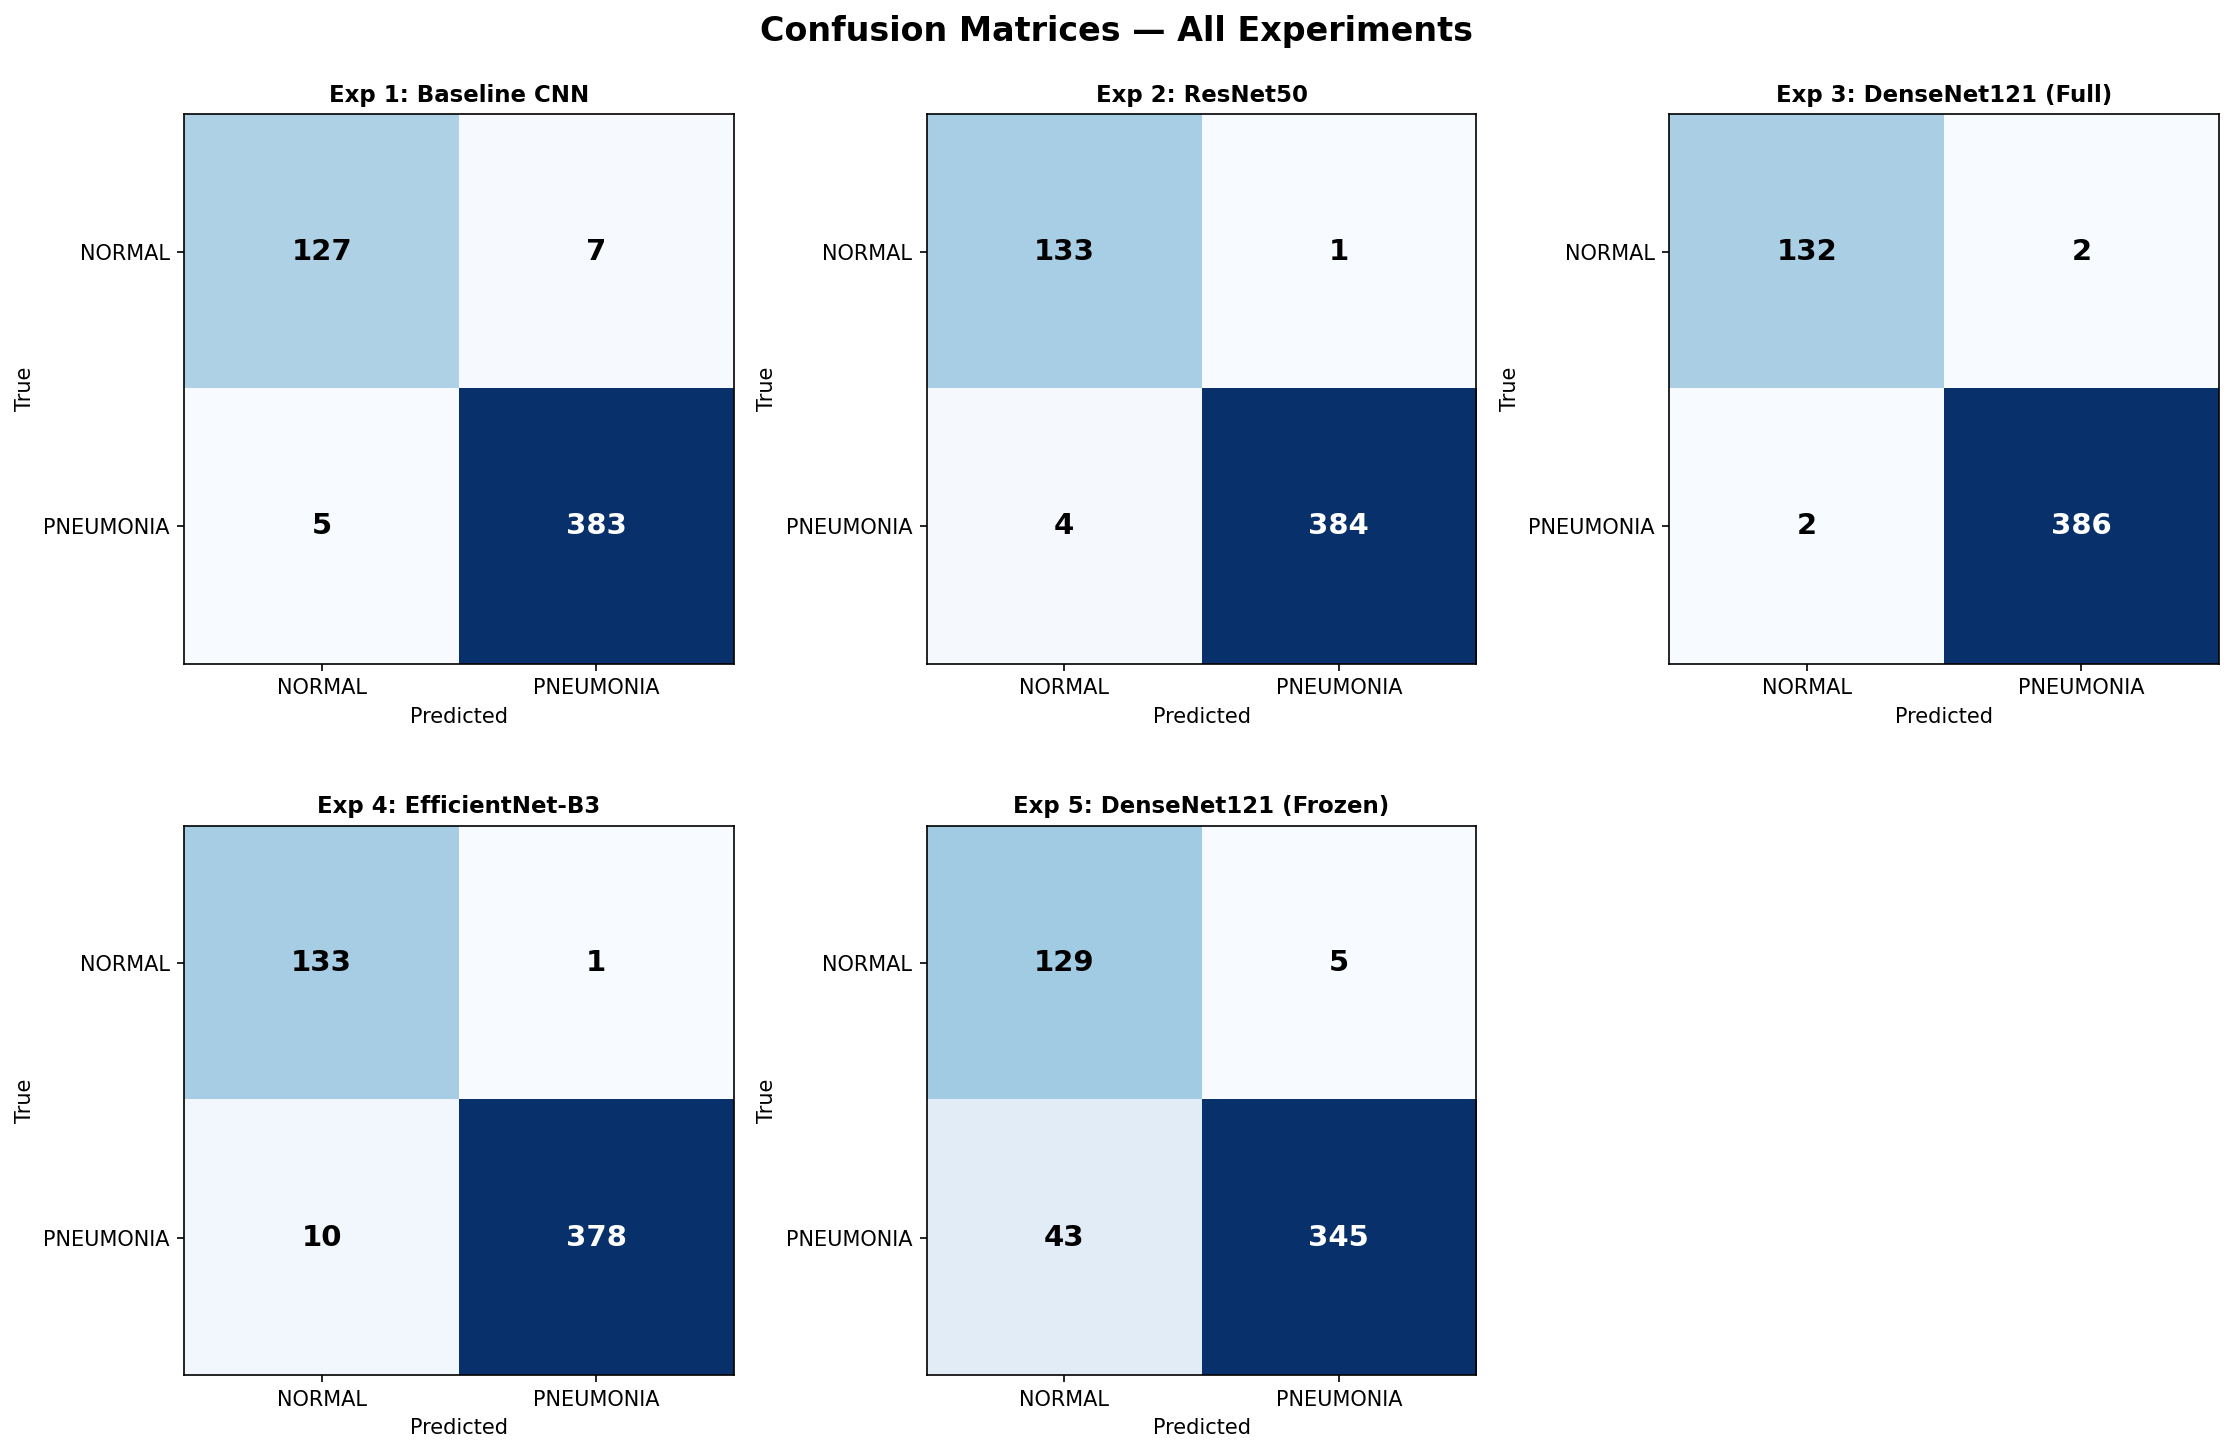
\includegraphics[width=\linewidth]{pneumonia_results/ml_experiments/confusion_matrices.png}
    \caption{Confusion matrices for all five experiments on the test set.}
    \label{fig:confusion}
\end{figure}

% Training curves
\begin{figure}[H]
    \centering
    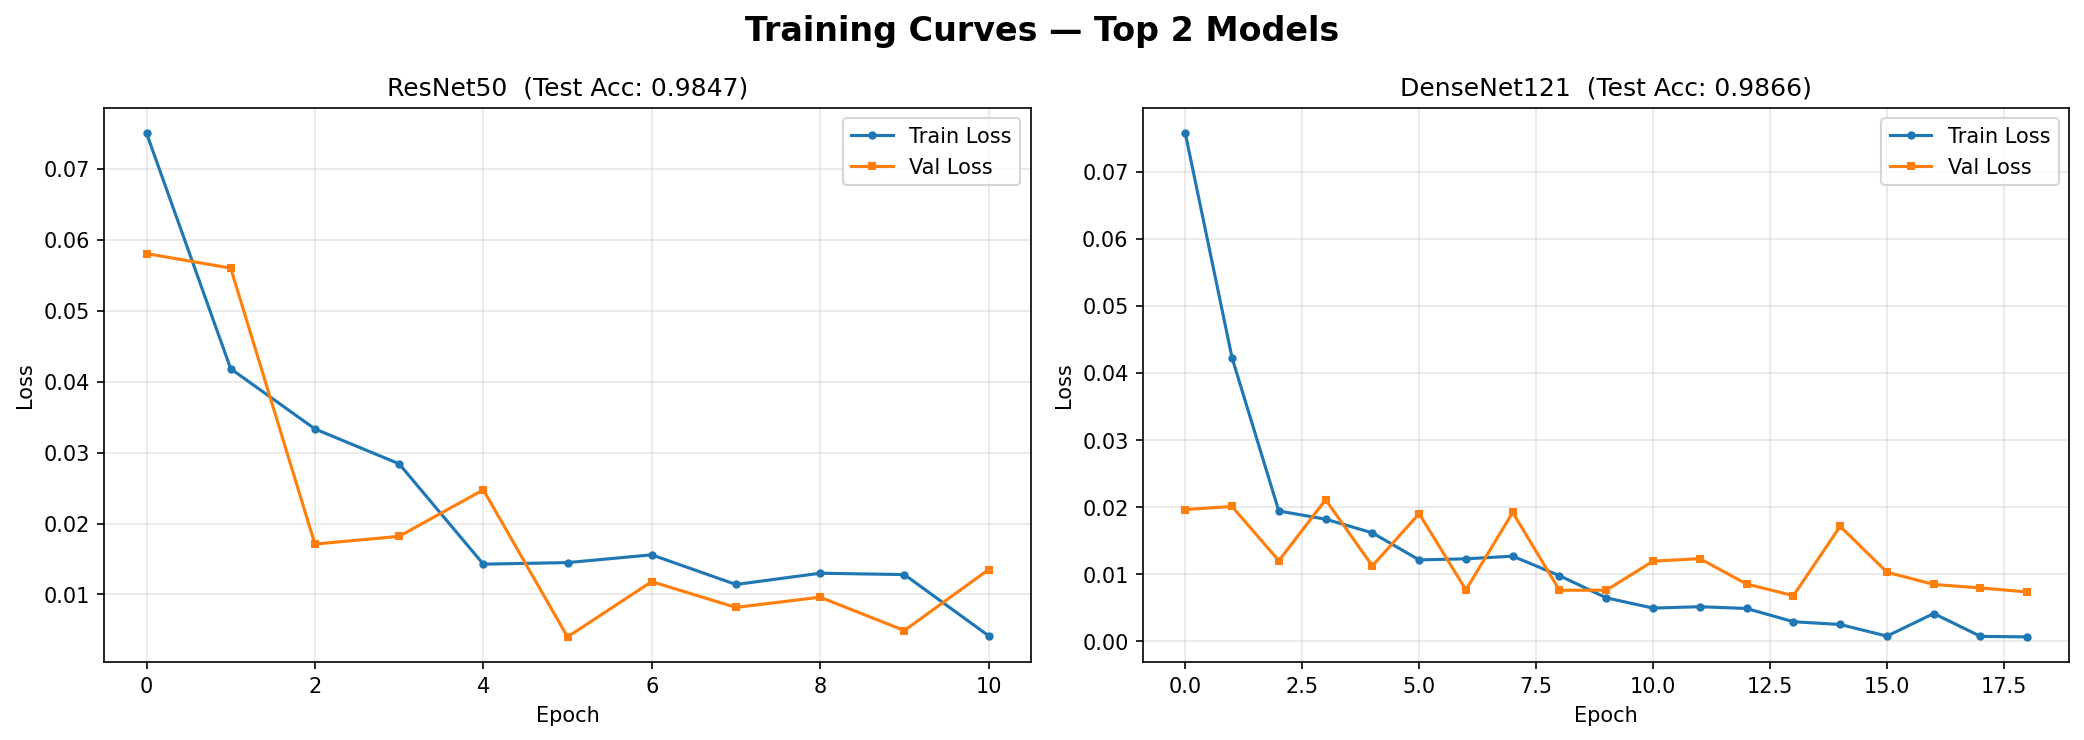
\includegraphics[width=\linewidth]{pneumonia_results/ml_experiments/training_curves.png}
    \caption{Training and validation loss curves for the top two performing
             experiments (selected automatically by test accuracy).}
    \label{fig:curves}
\end{figure}

% ─────────────────────────────────────────────────────────────────────────────
\newpage
\bibliographystyle{plain}
\begin{thebibliography}{99}

\bibitem{kanne2012chest}
Kanne, J.~P. (2012).
\textit{Chest CT findings in 2019 novel coronavirus (2019-nCoV) infections from Wuhan, China}.
Radiology, 295(1), 200--201.

\bibitem{gonzalez2018digital}
Gonzalez, R.~C., \& Woods, R.~E. (2018).
\textit{Digital Image Processing} (4th ed.).
Pearson.

\bibitem{kermany2018labeled}
Kermany, D.~S., et al. (2018).
Identifying medical diagnoses and treatable diseases by image-based deep learning.
\textit{Cell}, 172(5), 1122--1131.

\bibitem{king2001logistic}
King, G., \& Zeng, L. (2001).
Logistic regression in rare events data.
\textit{Political Analysis}, 9(2), 137--163.

\bibitem{krizhevsky2012imagenet}
Krizhevsky, A., Sutskever, I., \& Hinton, G.~E. (2012).
ImageNet classification with deep convolutional neural networks.
\textit{NeurIPS}, 25.

\bibitem{lecun1998gradient}
LeCun, Y., Bottou, L., Bengio, Y., \& Haffner, P. (1998).
Gradient-based learning applied to document recognition.
\textit{Proceedings of the IEEE}, 86(11), 2278--2324.

\bibitem{he2016deep}
He, K., Zhang, X., Ren, S., \& Sun, J. (2016).
Deep residual learning for image recognition.
\textit{CVPR}, 770--778.

\bibitem{huang2017densely}
Huang, G., Liu, Z., Van Der Maaten, L., \& Weinberger, K.~Q. (2017).
Densely connected convolutional networks.
\textit{CVPR}, 4700--4708.

\bibitem{rajpurkar2017chexnet}
Rajpurkar, P., et al. (2017).
CheXNet: Radiologist-level pneumonia detection on chest X-rays with deep learning.
\textit{arXiv:1711.05225}.

\bibitem{tan2019efficientnet}
Tan, M., \& Le, Q. (2019).
EfficientNet: Rethinking model scaling for convolutional neural networks.
\textit{ICML}, 6105--6114.

\bibitem{kingma2014adam}
Kingma, D.~P., \& Ba, J. (2015).
Adam: A method for stochastic optimization.
\textit{ICLR}.

\bibitem{yosinski2014transferable}
Yosinski, J., Clune, J., Bengio, Y., \& Lipson, H. (2014).
How transferable are features in deep neural networks?
\textit{NeurIPS}, 27.

\end{thebibliography}

\end{document}
